\documentclass[aspectratio=169, 11pt]{beamer}

% ============================================================
% Preambulo: tema, paquetes y estilos TikZ reutilizables
% ============================================================

\usepackage[spanish]{babel}
\usepackage[utf8]{inputenc}
\usepackage[T1]{fontenc}
\usepackage{graphicx}
\usepackage{booktabs}
\usepackage{array}
\usepackage{multicol}

% ---------- TikZ ----------
\usepackage{tikz}
\usetikzlibrary{arrows.meta, positioning, shapes.geometric, shapes.symbols,
                fit, backgrounds, calc, decorations.pathreplacing, chains,
                shadows, mindmap}

% ---------- Paleta institucional (IIEG) ----------
\definecolor{grispizarra}{HTML}{465055}   % Color institucional dominante: barras, paneles, encabezados
\definecolor{moradojalisco}{HTML}{6B2182} % Fondos de portada y separadores de sección
\definecolor{naranjajalisco}{HTML}{FF8300}% Branding exclusivo: escudos, íconos, comillas decorativas
\definecolor{grisclaro}{HTML}{F3F3F3}     % Fondo principal de slides de contenido
\definecolor{grisperla}{HTML}{EEF2F3}     % Variante de fondo en slides especiales

% ---------- Tema ----------
\usetheme{Madrid}
\usecolortheme{default}

% ---- Aplicación de la paleta institucional al tema Madrid ----
\setbeamercolor{palette primary}{bg=grispizarra,fg=white}
\setbeamercolor{palette secondary}{bg=moradojalisco,fg=white}
\setbeamercolor{palette tertiary}{bg=grispizarra,fg=white}
\setbeamercolor{palette quaternary}{bg=moradojalisco,fg=white}
\setbeamercolor{structure}{fg=moradojalisco}
\setbeamercolor{title}{fg=white,bg=moradojalisco}
\setbeamercolor{frametitle}{bg=grispizarra,fg=white}
\setbeamercolor{section in head/foot}{bg=moradojalisco,fg=white}
\setbeamercolor{author in head/foot}{bg=grispizarra,fg=white}
\setbeamercolor{normal text}{fg=black}
\setbeamercolor{block title}{bg=naranjajalisco,fg=black}
\setbeamercolor{block body}{bg=grisperla,fg=black}
\setbeamercolor{block title alerted}{bg=naranjajalisco,fg=black}
\setbeamercolor{block body alerted}{bg=grisperla,fg=black}

\setbeamertemplate{section in toc}[sections numbered]

% Paleta de colores del deck, derivada de la paleta institucional
% (se conservan los nombres usados en los diagramas TikZ de las secciones)
\colorlet{colPrimario}{grispizarra}
\colorlet{colSecundario}{moradojalisco}
\colorlet{colGris}{grispizarra}
\colorlet{colAgente}{moradojalisco}
\colorlet{colEntorno}{grispizarra}
\colorlet{colLLM}{naranjajalisco}
\colorlet{colHerramienta}{naranjajalisco!55!moradojalisco}
\colorlet{colAcento}{naranjajalisco!75!grispizarra}

% ---------- Estilos TikZ reutilizables en todo el deck ----------
\tikzset{
  cajaBase/.style={
    draw=colGris, thick, rounded corners=2pt,
    minimum height=1cm, minimum width=2.4cm,
    align=center, font=\small, text=colPrimario,
    fill=white, drop shadow
  },
  cajaAgente/.style={cajaBase, fill=colAgente!35},
  cajaEntorno/.style={cajaBase, fill=colEntorno!35},
  cajaLLM/.style={cajaBase, fill=colLLM!30},
  cajaHerramienta/.style={cajaBase, fill=colHerramienta!45},
  cajaAccento/.style={cajaBase, fill=colAcento!35},
  flecha/.style={-{Latex[length=2.2mm]}, thick, colGris},
  flechaDoble/.style={{Latex[length=2.2mm]}-{Latex[length=2.2mm]}, thick, colGris},
  flechaPunteada/.style={-{Latex[length=2.2mm]}, thick, dashed, colGris},
  etiquetaFlecha/.style={font=\scriptsize\itshape, text=colGris, fill=white, inner sep=1pt},
  nodoTiempo/.style={circle, draw=colSecundario, fill=colSecundario!25, thick,
    minimum size=8pt, inner sep=0pt},
}

% Comando corto para bloques de definicion resaltados
\newcommand{\definicion}[2]{%
  \begin{alertblock}{#1}
    #2
  \end{alertblock}
}

\newcommand{\slideimg}[1]{%
  \begin{center}
    \includegraphics[width=0.95\paperwidth,height=0.78\paperheight,keepaspectratio]{images/#1}
  \end{center}
}
\title{Agentes LLM}
\subtitle{}
\author{Ulises Moya}
\institute{IIEG, TSJ-Mario Molina}
\date{\today}
\logo{
\includegraphics[height=0.8cm]{images/iieg_logo.png}}


\begin{document}

\begin{frame}
  \titlepage
\end{frame}

\begin{frame}{Contenido}
  \tableofcontents
\end{frame}

% ============================================================
% Sección 0: Sobre mí (línea de tiempo de trayectoria)
% ============================================================

\begin{frame}{Sobre mí: trayectoria}
  \centering
  \begin{tikzpicture}[
      every node/.style={font=\scriptsize},
      etapa/.style={align=center, text width=1.9cm, font=\scriptsize}
    ]
    \draw[flecha, line width=1pt] (0,0) -- (12,0);

    \foreach \x/\lbl/\txt in {
        0/{2004}/{Lic. en Física\\(U. de Guadalajara)},
        2/{2007-13}/{MSc y PhD\\(UNAM / CINVESTAV)},
        4/{2017-18}/{Postdoc HPC+IA\\(Barcelona SC)},
        6/{2019-24}/{Director IA\\Gob. de Jalisco},
        8/{2020}/{Fulbright-García\\Robles (UT Dallas)},
        10/{2022-hoy}/{Consultor IA\\(World Bank, ...)},
        12/{2025-hoy}/{Director IA-HPC\\(IIEG)}
      }{
        \node[nodoTiempo] at (\x,0) {};
        \node[etapa, above=0.3cm] at (\x,0.3) {\lbl};
        \node[etapa] at (\x,-1.1) {\txt};
      }
  \end{tikzpicture}

  \vfill
  \small
  Ph.D. en Ingeniería Eléctrica · +65 publicaciones en IA para salud, clima y NLP \\
  Top 10 UNESCO-IRCAI Global 100 · Proyectos con OECD-GPAI, Banco Mundial y ONU
\end{frame}


\begin{frame}{Equipo de Trabajo}
\begin{center}
  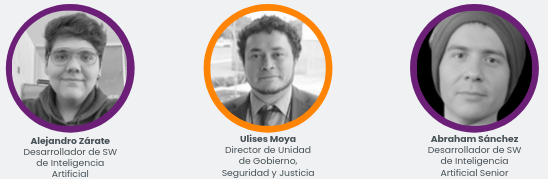
\includegraphics[width=0.45\paperwidth,height=0.38\paperheight,keepaspectratio]{images/team.png}
\end{center}
\end{frame}

% ============================================================
% Sección 1: Definición de agente
% ============================================================
\section{¿Qué es un agente?}

\begin{frame}{Una pregunta antes de empezar}
  \centering
  \Large
  ¿Qué tienen en común un termostato, \\
  un jugador de ajedrez artificial \\
  y ChatGPT usando un navegador?
  \vfill
  \normalsize
  \pause
  Los tres pueden describirse como \textbf{agentes}.
\end{frame}

\begin{frame}{Definición de agente}
  \definicion{Agente (Russell \& Norvig)}{
    Un agente es cualquier entidad que \textbf{percibe} su entorno a través
    de sensores y \textbf{actúa} sobre ese entorno a través de actuadores,
    con el fin de alcanzar un objetivo.
  }
  \vfill
  \begin{itemize}
    \item No requiere ``inteligencia''\, para ser agente: un termostato ya califica.
    \item Lo que lo hace \emph{interesante} es qué tan racional es su
      comportamiento frente al objetivo.
    \item Un \textbf{agente racional} elige, en cada instante, la acción que
      maximiza su desempeño esperado dado lo que ha percibido.
  \end{itemize}
\end{frame}

\begin{frame}{El ciclo agente–entorno}
  \centering
  \begin{tikzpicture}[node distance=2.2cm]
    \node[cajaAgente, minimum width=3.2cm, minimum height=1.6cm] (agente) {\textbf{AGENTE}\\[2pt]\footnotesize función/política};
    \node[cajaEntorno, minimum width=3.2cm, minimum height=1.6cm, right=4cm of agente] (entorno) {\textbf{ENTORNO}\\[2pt]\footnotesize mundo, tarea, usuario};

    \draw[flecha] (agente.30) -- ++(1.9,0) node[midway, above, etiquetaFlecha]{acción $a_t$} -- (entorno.150);
    \draw[flecha] (entorno.210) -- ++(-1.9,0) node[midway, below, etiquetaFlecha]{percepción $s_{t+1}$, recompensa $r_t$} -- (agente.-30);
  \end{tikzpicture}

  \vfill
  \begin{itemize}
    \item Sensores $\to$ estado percibido.
    \item Programa/política del agente $\to$ decide la acción.
    \item Actuadores $\to$ ejecutan la acción sobre el entorno.
    \item El entorno cambia, y el ciclo se repite.
  \end{itemize}
\end{frame}

\begin{frame}{Tipos clásicos de agentes (según su arquitectura)}
  \small
  \begin{itemize}
    \item \textbf{Reactivo simple}: regla condición-acción, sin memoria (termostato).
    \item \textbf{Basado en modelo}: mantiene un estado interno del mundo.
    \item \textbf{Basado en objetivos}: elige acciones que acercan a una meta.
    \item \textbf{Basado en utilidad}: pondera múltiples objetivos en conflicto.
    \item \textbf{Que aprende}: mejora su política con la experiencia (RL).
  \end{itemize}
  \vfill
  \begin{alertblock}{Adelanto}
    Un \textbf{agente LLM} añade una capa nueva: usa lenguaje natural como
    espacio de razonamiento interno, no solo como entrada/salida.
  \end{alertblock}
\end{frame}

% ============================================================
% Sección 2: Antecedentes / historia
% ============================================================
\section{Antecedentes e historia}

\begin{frame}{Línea de tiempo: de reglas a agentes que razonan}
  \centering
  \begin{tikzpicture}[
      every node/.style={font=\scriptsize},
      etapa/.style={align=center, text width=2.5cm, font=\scriptsize}
    ]
    \draw[flecha, line width=1pt] (0,0) -- (12,0);

    \foreach \x/\lbl/\txt in {
        0/{1950s-60s}/{Sistemas basados\\en reglas},
        2.4/{1980s}/{Sistemas\\expertos},
        4.8/{1990s}/{Agentes\\reactivos / RL\\tabular (Q-learning)},
        7.2/{2013-2016}/{Deep RL\\(DQN, AlphaGo)},
        9.6/{2017-2020}/{Transformers\\y LLMs (GPT)},
        12/{2022-hoy}/{Agentes LLM\\(ReAct, tool use,\\multiagente)}
      }{
        \node[nodoTiempo] at (\x,0) {};
        \node[etapa, above=0.3cm] at (\x,0.3) {\lbl};
        \node[etapa] at (\x,-1.1) {\txt};
      }
  \end{tikzpicture}
\end{frame}

\begin{frame}{Antes de los LLM: agentes simbólicos}
  \begin{itemize}
    \item \textbf{Sistemas expertos} (MYCIN, DENDRAL): reglas \texttt{si-entonces}
      escritas a mano por expertos humanos.
    \item \textbf{Planificación clásica} (STRIPS): buscar una secuencia de
      acciones que lleve de un estado inicial a una meta.
    \item \textbf{Agentes reactivos} (Brooks, robótica): sin representación
      interna del mundo, solo estímulo-respuesta.
    \item Limitación común: \textbf{frágiles} fuera del dominio para el que
      fueron programados; no generalizan.
  \end{itemize}
\end{frame}

\begin{frame}{El salto: aprendizaje y luego lenguaje}
  \centering
  \resizebox{!}{0.78\textheight}{%
  \begin{tikzpicture}[node distance=0.9cm]
    \node[cajaBase, fill=colGris!15] (a) {Reglas escritas a mano};
    \node[cajaBase, fill=colSecundario!25, below=of a] (b) {Aprendizaje por refuerzo\\(la política se aprende)};
    \node[cajaBase, fill=colLLM!30, below=of b] (c) {Modelos de lenguaje preentrenados\\(el conocimiento se aprende de texto)};
    \node[cajaAgente, below=of c] (d) {Agente LLM\\(razona en lenguaje + usa herramientas)};
    \draw[flecha] (a) -- (b);
    \draw[flecha] (b) -- (c);
    \draw[flecha] (c) -- (d);
  \end{tikzpicture}}
\end{frame}

\begin{frame}{Hitos recientes que habilitaron los agentes LLM}
  \small
  \begin{itemize}
    \item \textbf{2017} — \emph{Attention is All You Need}: arquitectura Transformer.
    \item \textbf{2020-2022} — GPT-3, InstructGPT: LLMs que \emph{siguen instrucciones}.
    \item \textbf{2022} — Paper \emph{ReAct}: intercalar razonamiento y acciones.
    \item \textbf{2023} — Explosión de frameworks: LangChain, AutoGPT, BabyAGI.
    \item \textbf{2024-2025} — Tool use nativo, MCP, modelos que ``razonan''
      (o1, DeepSeek-R1), SDKs de agentes de los propios labs.
  \end{itemize}
\end{frame}

\begin{frame}{Evolución de LLM como Herramienta}
  \begin{columns}[T]
    \begin{column}{0.5\textwidth}
      \textbf{Modelos Fundacionales}
      \begin{itemize}
        \item Predicciones de texto
        \item Limitaciones: falta de salidas estructuradas
      \end{itemize}
      \vspace{0.3cm}
      \textbf{Chats LLM}
      \begin{itemize}
        \item Sigue instrucciones conversacionales
        \item Limitaciones: propenso a alucinaciones, razonamiento limitado
      \end{itemize}
    \end{column}
    \begin{column}{0.5\textwidth}
      \textbf{LLM de Razonamiento}
      \begin{itemize}
        \item Procesa pasos de manera lógica
        \item Limitaciones: alto costo computacional
      \end{itemize}
      \vspace{0.3cm}
      \textbf{Agentes LLM}
      \begin{itemize}
        \item Detecta e integra conocimiento sobre herramientas externas
        \item Limitaciones: complejidad en implementación
      \end{itemize}
    \end{column}
  \end{columns}
\end{frame}


% ============================================================
% Sección 3: Aprendizaje por refuerzo
% ============================================================
\section{Aprendizaje por refuerzo}

\begin{frame}{¿Por qué hablar de RL en una charla de agentes LLM?}
  \begin{itemize}
    \item La palabra ``agente'' viene formalmente del \textbf{aprendizaje por
      refuerzo} (Reinforcement Learning, RL).
    \item RL es el marco matemático donde un agente aprende \emph{qué acción
      tomar} para maximizar una recompensa acumulada.
    \item Los LLMs modernos se afinan con una variante de RL
      (\textbf{RLHF}) — por eso el vocabulario de ``agente'', ``política''
      y ``recompensa'' reaparece constantemente.
  \end{itemize}
\end{frame}

\begin{frame}{El ciclo de RL}
  \centering
  \resizebox{!}{0.4\textheight}{%
  \begin{tikzpicture}[node distance=2.2cm]
    \node[cajaAgente, minimum width=3cm, minimum height=1.5cm] (agente) {\textbf{Agente}\\[2pt]\footnotesize política $\pi(a\mid s)$};
    \node[cajaEntorno, minimum width=3cm, minimum height=1.5cm, right=4.2cm of agente] (entorno) {\textbf{Entorno}};

    \draw[flecha] (agente.20) -- ++(2.2,0) node[midway, above, etiquetaFlecha]{acción $a_t$} -- (entorno.160);
    \draw[flecha] (entorno.200) -- ++(-2.2,0) node[midway, below, etiquetaFlecha]{estado $s_{t+1}$} -- (agente.-20);
    \draw[flecha] (entorno.-90) to[out=-90, in=-90, looseness=1.4]
      node[midway, below, etiquetaFlecha]{recompensa $r_t$} (agente.-90);
  \end{tikzpicture}}
  \vfill
  \begin{itemize}
    \item El agente busca la política $\pi$ que \textbf{maximiza la suma de
      recompensas} esperadas a largo plazo.
    \item Aprende por \textbf{prueba y error}: explora, observa el resultado,
      ajusta su política.
  \end{itemize}
\end{frame}

\begin{frame}{Ingredientes de un problema de RL}
  \small
  \begin{itemize}
    \item \textbf{Estado ($s$)}: descripción de la situación actual.
    \item \textbf{Acción ($a$)}: algo que el agente puede hacer.
    \item \textbf{Recompensa ($r$)}: señal numérica de qué tan buena fue la acción.
    \item \textbf{Política ($\pi$)}: la estrategia que mapea estados a acciones.
    \item \textbf{Valor ($V$, $Q$)}: qué tan bueno es un estado (o par estado-acción)
      a largo plazo.
  \end{itemize}
  \vfill
  \begin{exampleblock}{Ejemplo clásico}
    Un agente que juega Atari: estado = píxeles de la pantalla, acción =
    mover el joystick, recompensa = puntaje del juego.
  \end{exampleblock}
\end{frame}

\begin{frame}{De Q-learning a Deep RL}
  \begin{itemize}
    \item \textbf{Q-learning tabular}: guarda una tabla de valores
      $Q(s,a)$ — solo funciona con pocos estados posibles.
    \item \textbf{Deep RL} (DQN, PPO, etc.): una red neuronal
      \emph{aproxima} $Q$ o $\pi$ directamente — escala a espacios enormes
      (imágenes, texto).
    \item Hitos: \textbf{DQN} (Atari, 2013), \textbf{AlphaGo/AlphaZero}
      (2016-2017), \textbf{OpenAI Five}, \textbf{PPO} (algoritmo detrás de RLHF).
  \end{itemize}
\end{frame}

\begin{frame}{El puente hacia los LLM: RLHF}
  \centering
  \resizebox{!}{0.62\textheight}{%
  \begin{tikzpicture}[node distance=0.9cm]
    \node[cajaLLM] (modelo) {LLM preentrenado};
    \node[cajaHerramienta, below=of modelo] (sft) {Ajuste supervisado\\(ejemplos humanos)};
    \node[cajaAgente, below=of sft] (rm) {Modelo de recompensa\\(aprende preferencias humanas)};
    \node[cajaAccento, below=of rm] (ppo) {RL (PPO) contra\\el modelo de recompensa};
    \draw[flecha] (modelo) -- (sft);
    \draw[flecha] (sft) -- (rm);
    \draw[flecha] (rm) -- (ppo);
  \end{tikzpicture}}
  \vfill
  \small
  \textbf{RLHF} = \emph{Reinforcement Learning from Human Feedback}. Aquí el
  ``agente'' es el propio LLM y la ``recompensa'' viene de preferencias humanas.
\end{frame}

% ============================================================
% Sección 4: Agente vs Agente LLM
% ============================================================
\section{Agente clásico vs. agente LLM}

\begin{frame}{¿En qué se parecen?}
  \begin{itemize}
    \item Ambos siguen el ciclo \textbf{percibir $\to$ decidir $\to$ actuar}.
    \item Ambos operan dentro de un entorno (juego, sistema operativo,
      conversación, internet).
    \item Ambos pueden mejorar con retroalimentación.
  \end{itemize}
  \vfill
  \centering
  \Large ¿Entonces qué cambia?
\end{frame}

\begin{frame}{Diagrama comparativo}
  \centering
  \begin{tikzpicture}[node distance=0.9cm]
    % Agente clasico
    \node[cajaBase, fill=colGris!15, minimum width=4.6cm] (titulo1) {\textbf{Agente clásico (RL)}};
    \node[cajaAgente, below=of titulo1, minimum width=4.6cm] (pol) {Política $\pi(a|s)$\\aprendida por prueba/error};
    \node[cajaEntorno, below=of pol, minimum width=4.6cm] (acc) {Acciones discretas\\predefinidas por el entorno};

    % Agente LLM
    \node[cajaBase, fill=colGris!15, right=2.2cm of titulo1, minimum width=4.6cm] (titulo2) {\textbf{Agente LLM}};
    \node[cajaLLM, below=of titulo2, minimum width=4.6cm] (razon) {Razonamiento en lenguaje\\natural (chain-of-thought)};
    \node[cajaHerramienta, below=of razon, minimum width=4.6cm] (tools) {Acciones = llamadas a\\herramientas/funciones};

    \draw[flecha] (titulo1) -- (pol);
    \draw[flecha] (pol) -- (acc);
    \draw[flecha] (titulo2) -- (razon);
    \draw[flecha] (razon) -- (tools);
  \end{tikzpicture}
\end{frame}

\begin{frame}{Tabla comparativa}
  \small
  \begin{center}
  \begin{tabular}{@{}p{3.1cm}p{4.1cm}p{4.1cm}@{}}
    \toprule
    & \textbf{Agente clásico (RL)} & \textbf{Agente LLM} \\
    \midrule
    Cómo decide & Política numérica aprendida & Razonamiento en lenguaje (prompt) \\
    Cómo aprende & Prueba y error con recompensa & Preentrenado en texto + fine-tuning \\
    Espacio de acciones & Fijo, definido por el entorno & Abierto: cualquier herramienta con schema \\
    Adaptación a tareas nuevas & Requiere reentrenar & Cambia con el \emph{prompt}, sin reentrenar \\
    Explicabilidad & Baja (pesos numéricos) & Alta (razona en texto legible) \\
    \bottomrule
  \end{tabular}
  \end{center}
\end{frame}

\begin{frame}{Entonces, ¿qué es un agente LLM?}
  \definicion{Agente LLM}{
    Un sistema en el que un modelo de lenguaje \textbf{decide qué hacer a
    continuación} —incluyendo qué herramientas invocar y con qué
    argumentos— de forma iterativa, usando su propio razonamiento en
    lenguaje natural como ``memoria de trabajo'', hasta cumplir un objetivo.
  }
  \vfill
  \begin{itemize}
    \item El LLM cumple el rol de \textbf{política}: dado un estado
      (contexto), produce una acción (texto, tool call).
    \item Las \textbf{herramientas} amplían el entorno con el que puede
      interactuar (buscar, ejecutar código, leer archivos...).
  \end{itemize}
\end{frame}

% ============================================================
% Sección 5: Tipos de modelos LLM
% ============================================================
\section{Tipos de modelos LLM}

\begin{frame}{No todos los LLM son iguales}
  \begin{itemize}
    \item El mismo Transformer preentrenado puede terminar en productos muy
      distintos según cómo se \textbf{afine y se use}.
    \item Distinguimos al menos tres perfiles:
      \begin{enumerate}
        \item Modelo \textbf{base / funcional} (completion).
        \item Modelo \textbf{de chat} (instruction-tuned).
        \item Modelo \textbf{que razona} (reasoning model).
      \end{enumerate}
    \item Entender la diferencia importa porque \textbf{cada uno se comporta
      distinto dentro de un agente}.
  \end{itemize}
  \vfill
  \footnotesize Notebook de ejemplo: \url{https://colab.research.google.com/drive/1Q4bxbhWCD-PoDb2inHJTbSmeSjc9g16L?usp=sharing}
\end{frame}

\begin{frame}{1. Modelo base / funcional (completion)}
  \begin{itemize}
    \item Entrenado solo para \textbf{predecir el siguiente token} sobre un
      corpus masivo de texto.
    \item No sabe ``seguir instrucciones''\, ni ``conversar''\, — solo
      continúa el texto que se le da.
    \item Ejemplo de entrada: \texttt{``El capital de Francia es''}
      $\to$ continúa con \texttt{``París.''}
    \item Es la \textbf{materia prima}: casi nunca se usa directo en un
      producto, se afina después.
  \end{itemize}
  \begin{center}
    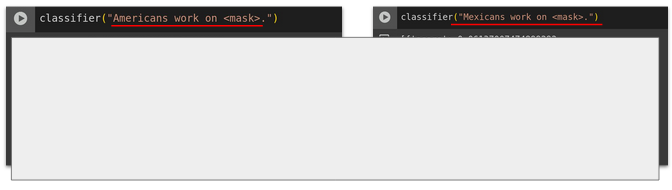
\includegraphics[width=0.85\textwidth]{images/bias_completion_ejemplo.png}
  \end{center}
\end{frame}

\begin{frame}{1. Modelo base / funcional (completion)}
  \begin{itemize}
    \item Entrenado solo para \textbf{predecir el siguiente token} sobre un
      corpus masivo de texto.
    \item No sabe ``seguir instrucciones''\, ni ``conversar''\, — solo
      continúa el texto que se le da.
    \item Ejemplo de entrada: \texttt{``El capital de Francia es''}
      $\to$ continúa con \texttt{``París.''}
    \item Es la \textbf{materia prima}: casi nunca se usa directo en un
      producto, se afina después.
  \end{itemize}
  \begin{center}
    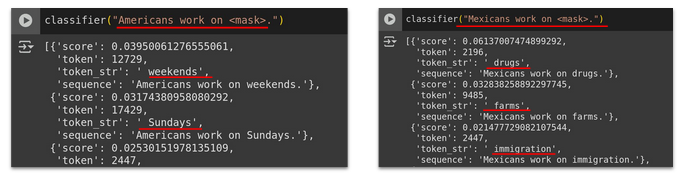
\includegraphics[width=0.85\textwidth]{images/bias_completion_ejemplo2.png}
  \end{center}
\end{frame}

\begin{frame}{2. Modelo de chat (instruction-tuned)}
  \begin{itemize}
    \item Se parte del modelo base y se afina con:
      \begin{itemize}
        \item Ejemplos de \textbf{instrucción $\to$ respuesta deseada} (SFT).
        \item \textbf{RLHF/DPO} para preferir respuestas útiles, seguras y
          bien formateadas.
      \end{itemize}
    \item Entiende roles (\texttt{system}, \texttt{user}, \texttt{assistant}).
    \item Es el formato que usan ChatGPT, Claude, Llama-chat, Qwen-instruct...
    \item Base de casi todos los agentes LLM actuales: necesitas que \emph{siga instrucciones}.
  \end{itemize}
\end{frame}

\begin{frame}{3. Modelo que razona (reasoning model)}
  \begin{itemize}
    \item Además del ajuste de chat, se entrena/afina para producir un
      \textbf{razonamiento extendido interno} antes de responder (ej. o1,
      DeepSeek-R1, Claude con \emph{extended thinking}).
    \item Ese razonamiento se optimiza (a menudo con RL) para llegar a
      respuestas correctas en tareas verificables (matemáticas, código).
    \item Trade-off: \textbf{más latencia y costo}, a cambio de mejor
      desempeño en tareas que requieren varios pasos lógicos.
  \end{itemize}
\end{frame}

\begin{frame}{Comparación de los tres pipelines}
  \centering
  \resizebox{\textwidth}{!}{%
  \begin{tikzpicture}[node distance=0.3cm, every node/.style={font=\scriptsize}]
    \tikzset{cajaBase/.append style={minimum height=0.65cm}}
    % Base
    \node[cajaBase, fill=colGris!15, minimum width=3.6cm] (b0) {Preentrenamiento};
    \node[cajaLLM, below=of b0, minimum width=3.6cm] (b1) {Modelo base\\(completion)};
    \node[below=of b1, minimum width=3.6cm, font=\scriptsize\itshape] (b2) {continúa texto};

    % Chat
    \node[cajaBase, fill=colGris!15, right=1.6cm of b0, minimum width=3.6cm] (c0) {Preentrenamiento};
    \node[cajaHerramienta, below=of c0, minimum width=3.6cm] (c1) {+ SFT + RLHF/DPO};
    \node[cajaLLM, below=of c1, minimum width=3.6cm] (c2) {Modelo de chat};
    \node[below=of c2, minimum width=3.6cm, font=\scriptsize\itshape] (c3) {sigue instrucciones};

    % Reasoning
    \node[cajaBase, fill=colGris!15, right=1.6cm of c0, minimum width=3.6cm] (r0) {Preentrenamiento};
    \node[cajaHerramienta, below=of r0, minimum width=3.6cm] (r1) {+ SFT + RLHF/DPO};
    \node[cajaAccento, below=of r1, minimum width=3.6cm] (r2) {+ RL sobre\\razonamiento paso a paso};
    \node[cajaLLM, below=of r2, minimum width=3.6cm] (r3) {Modelo que razona};
    \node[below=of r3, minimum width=3.6cm, font=\scriptsize\itshape] (r4) {piensa antes de responder};

    \draw[flecha] (b0)--(b1); \draw[flecha] (c0)--(c1); \draw[flecha] (c1)--(c2);
    \draw[flecha] (r0)--(r1); \draw[flecha] (r1)--(r2); \draw[flecha] (r2)--(r3);
  \end{tikzpicture}}
  \vfill
  \footnotesize Un agente LLM típico usa un modelo de \textbf{chat} con tool-calling;
  para tareas complejas de varios pasos conviene un modelo \textbf{que razona}.
\end{frame}

% ============================================================
% Sección 6: RAG
% ============================================================
\section{RAG: Retrieval-Augmented Generation}

\begin{frame}{El problema que resuelve RAG}
  \begin{itemize}
    \item Un LLM solo ``sabe'' lo que vio en su entrenamiento: conocimiento
      \textbf{congelado en el tiempo} y sin datos privados/internos.
    \item Alternativas para darle información nueva:
      \begin{enumerate}
        \item Reentrenar/afinar el modelo (caro, lento).
        \item Meter todo en el prompt (no escala, límite de contexto).
        \item \textbf{RAG}: buscar solo lo relevante y ponerlo en el prompt.
      \end{enumerate}
  \end{itemize}
  \vfill
  \definicion{RAG}{
    Recuperar información relevante de una fuente externa \emph{en el
    momento de la consulta} y dársela al LLM como contexto para generar
    la respuesta.
  }
\end{frame}

\begin{frame}{Pipeline de RAG}
  \centering
  \begin{tikzpicture}[node distance=1.5cm, every node/.style={font=\small}]
    \node[cajaAgente] (q) {Pregunta\\del usuario};
    \node[cajaLLM, right=of q] (emb) {Modelo de\\embeddings};
    \node[cajaHerramienta, right=of emb] (db) {Base vectorial\\(documentos)};
    \node[cajaEntorno, below=of db] (ctx) {Fragmentos\\relevantes};
    \node[cajaLLM, below=of emb] (llm) {LLM};
    \node[cajaAccento, below=of q] (resp) {Respuesta\\final};

    \draw[flecha] (q) -- (emb);
    \draw[flecha] (emb) -- node[above, etiquetaFlecha]{vector consulta} (db);
    \draw[flecha] (db) -- node[right, etiquetaFlecha]{top-$k$ similares} (ctx);
    \draw[flecha] (ctx) -- (llm);
    \draw[flecha] (q) to[bend left=15] (llm);
    \draw[flecha] (llm) -- (resp);
  \end{tikzpicture}
  \vfill
  \footnotesize La pregunta viaja por dos caminos: se usa para \textbf{buscar}
  y se usa (junto al contexto recuperado) para \textbf{generar} la respuesta.
\end{frame}

\begin{frame}{¿Qué es un embedding, en una frase?}
  \definicion{Embedding}{
    Un vector de números que representa el \emph{significado} de un texto,
    de forma que textos con significado parecido quedan cerca en ese
    espacio vectorial.
  }
  \vfill
  \begin{itemize}
    \item Se indexan todos los documentos (o fragmentos/\emph{chunks}) como
      embeddings en una \textbf{base vectorial} (FAISS, Chroma, pgvector...).
    \item En consulta: se calcula el embedding de la pregunta y se busca por
      \textbf{similitud} (coseno) los fragmentos más cercanos.
  \end{itemize}
\end{frame}

\begin{frame}{Ejemplo 1: asistente sobre documentación interna}
  \small
  \begin{enumerate}
    \item Se indexan los manuales/wiki de la empresa en chunks de \textasciitilde500 tokens.
    \item Usuario pregunta: \emph{``¿Cuántos días de vacaciones tengo el primer año?''}
    \item Se recuperan los 3 fragmentos del manual de RR.HH. más relevantes.
    \item El LLM responde \textbf{citando} esos fragmentos, sin inventar la política.
  \end{enumerate}
  \vfill
  \begin{alertblock}{Por qué importa}
    Sin RAG, el modelo alucinaría una cifra genérica; con RAG, responde con
    la política \emph{real} de la empresa.
  \end{alertblock}
\end{frame}

\begin{frame}{Ejemplo 2: RAG dentro de un agente}
  \small
  \begin{enumerate}
    \item El agente recibe: \emph{``Resume los cambios de la última versión
      de nuestra librería''}.
    \item El agente decide llamar a la herramienta \texttt{buscar\_docs(query)}.
    \item La herramienta hace la recuperación (RAG) y devuelve fragmentos del changelog.
    \item El agente redacta el resumen usando esos fragmentos como evidencia.
  \end{enumerate}
  \vfill
  RAG aquí \textbf{no es un paso fijo}: es una herramienta más que el agente
  decide usar cuando la necesita.
\end{frame}

\begin{frame}{Retos comunes de RAG}
  \begin{itemize}
    \item \textbf{Chunking}: fragmentos muy grandes pierden precisión, muy
      chicos pierden contexto.
    \item \textbf{Recuperación pobre} = respuesta pobre, aunque el LLM sea excelente.
    \item Combinar búsqueda \textbf{semántica + por palabras clave} (\emph{hybrid search})
      suele dar mejores resultados.
    \item \emph{Re-ranking}: recuperar más candidatos y luego reordenar los
      mejores con un modelo más preciso (y más caro).
  \end{itemize}
\end{frame}

% ============================================================
% Sección 7: Chain-of-Thought y ReAct
% ============================================================
\section{Chain-of-Thought y ReAct}

\begin{frame}{Chain-of-Thought (CoT)}
  \definicion{Chain-of-Thought}{
    Técnica de \emph{prompting} donde se pide (o se induce) al modelo a
    escribir su \textbf{razonamiento paso a paso} antes de dar la respuesta
    final, en lugar de responder directo.
  }
  \vfill
  \begin{itemize}
    \item Simple de aplicar: basta agregar ``pensemos paso a paso''\, al prompt.
    \item Mejora notablemente el desempeño en tareas de \textbf{lógica,
      matemáticas y problemas de varios pasos}.
    \item Es la base conceptual de los modelos ``que razonan''\ (sección anterior).
  \end{itemize}
\end{frame}

\begin{frame}{CoT en un diagrama}
  \centering
  \begin{tikzpicture}[node distance=0.5cm]
    \node[cajaAgente] (p) {Pregunta};
    \node[cajaLLM, below=of p, minimum width=6cm, minimum height=1.6cm] (r) {
      \begin{minipage}{5.4cm}\scriptsize
        \textbf{Razonamiento:} ``Primero calculo X, luego uso ese valor
        para obtener Y, y con eso...''
      \end{minipage}};
    \node[cajaAccento, below=of r] (a) {Respuesta final};
    \draw[flecha] (p) -- (r);
    \draw[flecha] (r) -- (a);
  \end{tikzpicture}
  \vfill
  \footnotesize CoT es puro \emph{razonamiento en texto} — todavía no
  interactúa con el mundo exterior.
\end{frame}

\begin{frame}{La limitación de CoT}
  \begin{itemize}
    \item CoT razona muy bien \textbf{sobre lo que ya sabe}.
    \item Pero no puede verificar hechos, hacer cálculos exactos grandes,
      ni consultar información nueva — solo ``piensa en voz alta''.
    \item ¿Qué pasa si el razonamiento necesita un dato externo
      (una búsqueda, un cálculo, un archivo)?
  \end{itemize}
  \vfill
  \centering
  \Large $\Rightarrow$ ReAct
\end{frame}

\begin{frame}{ReAct: Reasoning + Acting}
  \definicion{ReAct (Yao et al., 2022)}{
    Intercalar pasos de \textbf{razonamiento} (Thought) con pasos de
    \textbf{acción} (Action) sobre herramientas externas, observando el
    resultado (Observation) antes de continuar razonando.
  }
  \vfill
  \small
  \texttt{Thought} $\to$ \texttt{Action} $\to$ \texttt{Observation} $\to$
  \texttt{Thought} $\to$ \dots $\to$ \texttt{Respuesta final}
\end{frame}

\begin{frame}{El loop ReAct}
  \centering
  \begin{tikzpicture}[node distance=1.1cm]
    \node[cajaLLM] (t) {\textbf{Thought}\\¿qué necesito hacer?};
    \node[cajaHerramienta, right=1.8cm of t] (a) {\textbf{Action}\\llamar herramienta};
    \node[cajaEntorno, below=of a] (o) {\textbf{Observation}\\resultado obtenido};
    \node[cajaLLM, below=of t] (t2) {\textbf{Thought}\\¿ya tengo la respuesta?};

    \draw[flecha] (t) -- (a);
    \draw[flecha] (a) -- (o);
    \draw[flecha] (o) -- (t2);
    \draw[flecha] (t2.west) to[out=180,in=180,looseness=1.3] node[left, etiquetaFlecha, align=center]{repetir\\si falta info} (t.west);
    \node[cajaAccento, below=of t2] (fin) {Respuesta final};
    \draw[flecha] (t2) -- node[right, etiquetaFlecha]{si ya alcanza} (fin);
  \end{tikzpicture}
\end{frame}

\begin{frame}{Ejemplo de traza ReAct}
  \footnotesize
  \begin{block}{Pregunta}
    ``¿Qué día de la semana cae el 25 de diciembre de este año, y a cuánto
    equivale en horas si faltan 40 días?''
  \end{block}
  \begin{itemize}
    \item \texttt{Thought}: necesito saber la fecha de hoy.
    \item \texttt{Action}: \texttt{fecha\_actual()}
    \item \texttt{Observation}: \texttt{"2026-07-02"}
    \item \texttt{Thought}: ahora calculo los días restantes y la conversión.
    \item \texttt{Action}: \texttt{calculadora("40 * 24")}
    \item \texttt{Observation}: \texttt{960}
    \item \texttt{Thought}: ya puedo responder.
    \item \textbf{Respuesta final}: ``Faltan 960 horas; el 25 de diciembre es viernes.''
  \end{itemize}
\end{frame}

% ============================================================
% Sección 8: Automatización de procesos de código
% ============================================================
\section{Automatizar procesos de código con agentes}

\begin{frame}{De autocompletado a agente de código}
  \begin{itemize}
    \item \textbf{Autocompletado} (Copilot clásico): sugiere la siguiente
      línea, el humano decide todo lo demás.
    \item \textbf{Agente de código} (Claude Code, Cursor Agent, Devin...):
      puede \emph{planear, escribir, ejecutar, ver el error y corregir} —
      todo en un loop, con supervisión humana en distintos grados.
    \item La diferencia clave: el agente tiene \textbf{herramientas} para
      leer/escribir archivos y \textbf{ejecutar} lo que escribe.
  \end{itemize}
\end{frame}

\begin{frame}{El loop generar-ejecutar-corregir}
  \centering
  \begin{tikzpicture}[node distance=1.2cm]
    \node[cajaLLM] (gen) {Generar/editar código};
    \node[cajaHerramienta, right=2cm of gen] (run) {Ejecutar\\(tests, linter, script)};
    \node[cajaEntorno, below=of run] (obs) {Observar salida\\(error, stack trace)};
    \node[cajaAccento, below=of gen] (fin) {¿Pasa? $\to$ Terminar};

    \draw[flecha] (gen) -- (run);
    \draw[flecha] (run) -- (obs);
    \draw[flecha] (obs) -- node[below, etiquetaFlecha]{si falla, corregir} (gen);
    \draw[flecha] (obs) -- node[right, etiquetaFlecha]{si pasa} (fin);
  \end{tikzpicture}
  \vfill
  \footnotesize Este es, literalmente, ReAct aplicado a ingeniería de software:
  \texttt{Thought} (qué cambiar) $\to$ \texttt{Action} (editar/ejecutar) $\to$
  \texttt{Observation} (resultado).
\end{frame}

\begin{frame}{Ejemplos de tareas automatizables}
  \small
  \begin{itemize}
    \item \textbf{Refactors mecánicos a escala}: renombrar una función y
      actualizar todos sus usos en un repo grande.
    \item \textbf{Corrección de bugs guiada por tests}: correr la suite,
      leer el fallo, editar, repetir hasta que pase.
    \item \textbf{Generación de código repetitivo}: boilerplate, migraciones,
      adaptadores entre APIs.
    \item \textbf{Revisión de código}: detectar bugs, sugerir simplificaciones
      antes de mergear.
    \item \textbf{Automatización de CI/CD}: diagnosticar por qué falló un
      pipeline y proponer el fix.
  \end{itemize}
\end{frame}

\begin{frame}{Qué necesita un agente para hacer esto bien}
  \begin{itemize}
    \item Acceso de \textbf{lectura/escritura} al sistema de archivos.
    \item Una forma de \textbf{ejecutar comandos} (shell, tests, build).
    \item \textbf{Feedback verificable}: tests, linters, tipos — señales
      objetivas de si el cambio funcionó (no solo ``se ve bien'').
    \item \textbf{Límites y supervisión}: permisos, sandboxing, confirmación
      humana en acciones riesgosas (borrar, hacer push, etc.).
  \end{itemize}
\end{frame}

\begin{frame}{Riesgos a tener en cuenta}
  \begin{alertblock}{No es magia, hay que vigilarlo}
    \begin{itemize}
      \item Puede ``arreglar'' el síntoma y no la causa si el feedback es débil.
      \item Puede ejecutar comandos destructivos si no hay barreras.
      \item Requiere buen criterio sobre \textbf{qué automatizar sin supervisión}
        y qué requiere aprobación humana explícita.
    \end{itemize}
  \end{alertblock}
\end{frame}

% ============================================================
% Sección 9: Frameworks de agentes (breve)
% ============================================================
\section{Frameworks de agentes}

\begin{frame}{¿Para qué sirve un framework de agentes?}
  \begin{itemize}
    \item Resuelven en común: manejo de historial, parsing de tool calls,
      loops de agente, memoria, orquestación multiagente.
    \item No son estrictamente necesarios (un loop ReAct se puede escribir
      a mano, como veremos en la demo) — pero ahorran trabajo repetitivo
      en proyectos grandes.
    \item Riesgo: añaden \textbf{abstracción y dependencias}; a veces
      conviene empezar simple y adoptar un framework solo cuando se
      necesita.
  \end{itemize}
\end{frame}

\begin{frame}{Panorama de frameworks (2026)}
  \small
  \begin{center}
  \begin{tabular}{@{}p{2.6cm}p{5.6cm}@{}}
    \toprule
    \textbf{Framework} & \textbf{Enfoque principal} \\
    \midrule
    LangChain / LangGraph & Cadenas de LLM + grafos de estados explícitos para agentes complejos \\
    CrewAI & Equipos de agentes con roles definidos (multiagente) \\
    AutoGen / AG2 (Microsoft) & Conversaciones entre múltiples agentes \\
    OpenAI Agents SDK & Agentes ligeros con \emph{handoffs} entre ellos \\
    Claude Agent SDK & El mismo motor de agente detrás de Claude Code, reusable en tus apps \\
    \bottomrule
  \end{tabular}
  \end{center}
\end{frame}

\begin{frame}{¿Framework o loop a mano?}
  \centering
  \resizebox{\textwidth}{!}{%
  \begin{tikzpicture}[node distance=1cm]
    \node[cajaAgente, minimum width=5cm] (simple) {Tarea simple, 1 agente, pocas herramientas};
    \node[cajaHerramienta, below=of simple, minimum width=5cm] (mano) {$\to$ loop ReAct escrito a mano};
    \node[cajaAccento, right=2.5cm of simple, minimum width=5cm] (compleja) {Multiagente, memoria persistente, orquestación};
    \node[cajaLLM, below=of compleja, minimum width=5cm] (fw) {$\to$ framework (LangGraph, CrewAI...)};
    \draw[flecha] (simple) -- (mano);
    \draw[flecha] (compleja) -- (fw);
  \end{tikzpicture}}
  \vfill
  \footnotesize En esta charla construimos el caso simple: entender el loop
  antes de delegarlo a un framework.
\end{frame}

\begin{frame}{Protocolo común: Model Context Protocol (MCP)}
  \begin{itemize}
    \item Estándar abierto (Anthropic, 2024) para conectar un LLM con
      \textbf{herramientas y fuentes de datos} de forma uniforme.
    \item Antes: cada integración era un conector distinto por framework.
    \item Con MCP: un servidor de herramientas puede usarse desde cualquier
      cliente/agente compatible (Claude, editores, otros frameworks).
    \item Ayuda a que el ecosistema de herramientas \textbf{no dependa de
      un solo framework}.
  \end{itemize}
\end{frame}

% ============================================================
% Sección 10: Sistemas multiagente
% ============================================================
\section{Sistemas multiagente}

\begin{frame}{¿Por qué usar varios agentes?}
  \begin{itemize}
    \item Un solo agente con demasiadas responsabilidades tiende a
      \textbf{perder foco} (contexto saturado, instrucciones contradictorias).
    \item Dividir el trabajo entre agentes \textbf{especializados}
      —cada uno con su propio prompt, herramientas y contexto— suele dar
      mejores resultados en tareas grandes.
    \item Costo: más complejidad, más latencia, más tokens.
  \end{itemize}
\end{frame}

\begin{frame}{Topología 1: orquestador–trabajadores}
  \centering
  \begin{tikzpicture}[node distance=1.6cm]
    \node[cajaAccento] (orq) {Orquestador};
    \node[cajaAgente, below left=1.4cm and 1.6cm of orq] (w1) {Trabajador 1};
    \node[cajaAgente, below=1.6cm of orq] (w2) {Trabajador 2};
    \node[cajaAgente, below right=1.4cm and 1.6cm of orq] (w3) {Trabajador 3};
    \draw[flecha] (orq) -- (w1);
    \draw[flecha] (orq) -- (w2);
    \draw[flecha] (orq) -- (w3);
    \draw[flechaPunteada] (w1) to[bend right=15] (orq);
    \draw[flechaPunteada] (w3) to[bend left=15] (orq);
  \end{tikzpicture}
  \vfill
  \footnotesize Un agente central descompone la tarea, la reparte y
  \textbf{combina los resultados}. Ideal cuando las subtareas son
  independientes entre sí.
\end{frame}

\begin{frame}{Topología 2: pipeline secuencial}
  \centering
  \begin{tikzpicture}[node distance=1.8cm]
    \node[cajaAgente] (a1) {Agente\\investigador};
    \node[cajaAgente, right=of a1] (a2) {Agente\\redactor};
    \node[cajaAgente, right=of a2] (a3) {Agente\\revisor};
    \draw[flecha] (a1) -- (a2);
    \draw[flecha] (a2) -- (a3);
  \end{tikzpicture}
  \vfill
  \footnotesize Cada agente recibe la salida del anterior como entrada.
  Bueno para procesos con \textbf{etapas claras} (investigar $\to$ escribir
  $\to$ corregir).
\end{frame}

\begin{frame}{Topología 3: colaborativa / debate}
  \centering
  \begin{tikzpicture}[node distance=2.4cm]
    \node[cajaAgente] (a1) {Agente A};
    \node[cajaAgente, right=of a1] (a2) {Agente B};
    \node[cajaAccento, below=1.2cm of $(a1)!0.5!(a2)$] (j) {Juez / síntesis};
    \draw[flechaDoble] (a1) -- (a2);
    \draw[flecha] (a1) -- (j);
    \draw[flecha] (a2) -- (j);
  \end{tikzpicture}
  \vfill
  \footnotesize Los agentes discuten/critican propuestas entre sí antes de
  llegar a una respuesta final — útil para \textbf{decisiones que se
  benefician de puntos de vista distintos}.
\end{frame}

\begin{frame}{Riesgos propios de multiagente}
  \begin{itemize}
    \item \textbf{Costos y latencia} se multiplican por cada agente involucrado.
    \item \textbf{Errores en cascada}: un agente con información incorrecta
      contamina a los que dependen de él.
    \item Coordinación: decidir \emph{cuándo termina} cada agente y qué
      formato usan para comunicarse entre sí.
    \item Regla práctica: usar multiagente solo cuando un solo agente
      \textbf{ya demostró} no ser suficiente.
  \end{itemize}
\end{frame}

% ============================================================
% Sección 11: Patrones de diseño agénticos
% ============================================================
\section{Patrones de diseño agénticos}

\begin{frame}{Cuatro patrones recurrentes}
  \begin{enumerate}
    \item \textbf{Reflection} (auto-crítica)
    \item \textbf{Planning} (planeación)
    \item \textbf{Tool use} (uso de herramientas)
    \item \textbf{Multi-agent collaboration} (colaboración multiagente)
  \end{enumerate}
  \vfill
  \footnotesize Popularizados por Andrew Ng / DeepLearning.AI como los
  bloques básicos con los que se construye casi cualquier sistema agéntico.
\end{frame}

\begin{frame}{Patrón: Reflection}
  \centering
  \begin{tikzpicture}[node distance=1.4cm]
    \node[cajaLLM] (gen) {Generar respuesta/borrador};
    \node[cajaAccento, right=2.2cm of gen] (crit) {Autocriticar\\(el mismo u otro LLM)};
    \node[cajaAgente, below=of gen] (fin) {Versión mejorada};
    \draw[flecha] (gen) -- (crit);
    \draw[flecha] (crit) -- node[right, etiquetaFlecha]{feedback} (fin);
    \draw[flechaPunteada] (fin.west) to[out=180,in=180, looseness=1.2] (gen.west);
  \end{tikzpicture}
  \vfill
  \footnotesize El agente revisa su propio trabajo antes de entregarlo —
  como un borrador y su edición.
\end{frame}

\begin{frame}{Patrón: Planning}
  \centering
  \resizebox{!}{0.58\textheight}{%
  \begin{tikzpicture}[node distance=0.7cm]
    \node[cajaAgente] (obj) {Objetivo complejo};
    \node[cajaLLM, below=of obj] (plan) {Descomponer en subtareas};
    \node[cajaHerramienta, below=of plan] (s1) {Subtarea 1 $\to$ 2 $\to$ 3 \dots};
    \node[cajaAccento, below=of s1] (fin) {Ejecutar y combinar};
    \draw[flecha] (obj) -- (plan);
    \draw[flecha] (plan) -- (s1);
    \draw[flecha] (s1) -- (fin);
  \end{tikzpicture}}
  \vfill
  \footnotesize El agente traza un plan \emph{antes} de actuar, en vez de
  improvisar acción por acción.
\end{frame}

\begin{frame}{Patrón: Tool use}
  \centering
  \begin{tikzpicture}[node distance=1.6cm]
    \node[cajaLLM] (llm) {LLM};
    \node[cajaHerramienta, above right=0.8cm and 2cm of llm] (t1) {Calculadora};
    \node[cajaHerramienta, right=2cm of llm] (t2) {Buscador};
    \node[cajaHerramienta, below right=0.8cm and 2cm of llm] (t3) {Ejecutor de código};
    \draw[flechaDoble] (llm) -- (t1);
    \draw[flechaDoble] (llm) -- (t2);
    \draw[flechaDoble] (llm) -- (t3);
  \end{tikzpicture}
  \vfill
  \footnotesize El patrón que ya vimos en RAG y ReAct: el LLM decide
  \emph{cuándo} y \emph{con qué argumentos} invocar cada herramienta.
\end{frame}

\begin{frame}{Patrón: Multi-agent collaboration}
  \centering
  \footnotesize Ya visto en la sección anterior: orquestador-trabajadores,
  pipeline, debate.
  \vfill
  \begin{itemize}
    \item Se combina con los otros tres: cada agente puede tener su propio
      ciclo de \emph{planning + tool use + reflection}.
    \item Es el patrón de \textbf{mayor nivel}: compone a los demás.
  \end{itemize}
\end{frame}

\begin{frame}{Los cuatro patrones combinados}
  \centering
  \resizebox{0.8\textwidth}{0.48\textheight}{%
  \begin{tikzpicture}[node distance=0.9cm]
    \node[cajaBase, fill=colGris!15, minimum width=8.5cm] (top) {\textbf{Multi-agent collaboration}};
    \node[cajaAgente, below=of top, minimum width=2.5cm] (p1) {Planning};
    \node[cajaHerramienta, right=0.4cm of p1, minimum width=2.5cm] (p2) {Tool use};
    \node[cajaAccento, right=0.4cm of p2, minimum width=2.5cm] (p3) {Reflection};
    \draw[flecha] (top.south) -- ++(0,-0.3) -| (p1.north);
    \draw[flecha] (top.south) -- (p2.north);
    \draw[flecha] (top.south) -- ++(0,-0.3) -| (p3.north);
  \end{tikzpicture}}
  \vfill
  \footnotesize En la práctica, un buen agente combina varios de estos
  patrones a la vez, no uno solo.
\end{frame}

% ============================================================
% Sección 12: Herramientas de agentes
% ============================================================
\section{Herramientas de agentes}

\begin{frame}{¿Qué es una ``herramienta'' para un LLM?}
  \definicion{Tool / function calling}{
    Una función externa que el LLM puede invocar, descrita mediante un
    \textbf{schema} (nombre, descripción, parámetros) que el modelo usa
    para decidir cuándo y cómo llamarla.
  }
  \vfill
  \begin{itemize}
    \item El LLM \textbf{no ejecuta la función}: solo genera la
      \emph{intención} de llamarla (nombre + argumentos en JSON).
    \item El programa que envuelve al LLM es quien \textbf{ejecuta} la
      función real y le devuelve el resultado.
  \end{itemize}
\end{frame}

\begin{frame}[fragile]{Anatomía de un tool schema}
  \footnotesize
\begin{verbatim}
{
  "name": "calculadora",
  "description": "Evalua una expresion aritmetica",
  "parameters": {
    "type": "object",
    "properties": {
      "expresion": {"type": "string"}
    },
    "required": ["expresion"]
  }
}
\end{verbatim}
  \vfill
  \normalsize El modelo elige el nombre y llena los parámetros; tu código
  ejecuta \texttt{calculadora(expresion="3*7")}.
\end{frame}

\begin{frame}{Categorías de herramientas comunes}
  \small
  \begin{itemize}
    \item \textbf{Cómputo}: calculadora, intérprete de código (Python, SQL).
    \item \textbf{Información}: búsqueda web, RAG sobre documentos, APIs.
    \item \textbf{Sistema de archivos}: leer/escribir/editar archivos.
    \item \textbf{Acciones externas}: enviar correos, crear tickets, llamar APIs de terceros.
    \item \textbf{Memoria}: guardar/recuperar notas entre sesiones.
  \end{itemize}
\end{frame}

\begin{frame}{MCP: estandarizando las herramientas}
  \begin{itemize}
    \item \textbf{Model Context Protocol}: un servidor MCP expone un set de
      herramientas de forma estándar, consumible por cualquier cliente compatible.
    \item Ventaja: escribes la herramienta \textbf{una vez}, se conecta a
      Claude, a un IDE, o a cualquier agente que hable MCP.
    \item Es el equivalente a lo que USB hizo con los periféricos: un
      conector común en vez de uno distinto por dispositivo.
  \end{itemize}
\end{frame}

% ============================================================
% Sección 13: Puente a la demo práctica
% ============================================================
\section{Demo: un agente simple con LLM local}

\begin{frame}{Lo que vamos a construir}
  \begin{itemize}
    \item Un agente \textbf{mínimo} corriendo 100\% local con
      \href{https://ollama.com}{Ollama} — sin llaves de API, sin costo.
    \item Tres herramientas simples: \texttt{calculadora}, \texttt{fecha\_actual},
      \texttt{leer\_archivo}.
    \item El ciclo \textbf{ReAct} que ya vimos, implementado en \textasciitilde100
      líneas de Python: sin frameworks, para entender cada pieza.
  \end{itemize}
\end{frame}

\begin{frame}{Arquitectura de la demo}
  \centering
  \begin{tikzpicture}[node distance=1.4cm]
    \node[cajaAgente] (user) {Pregunta del usuario};
    \node[cajaLLM, below=of user] (ollama) {Ollama (modelo local)\\con tool-calling};
    \node[cajaHerramienta, right=2.2cm of ollama] (tools) {calculadora\\fecha\_actual\\leer\_archivo};
    \node[cajaAccento, below=of ollama] (resp) {Respuesta final};

    \draw[flecha] (user) -- (ollama);
    \draw[flechaDoble] (ollama) -- node[above, etiquetaFlecha]{tool call / resultado} (tools);
    \draw[flecha] (ollama) -- (resp);
  \end{tikzpicture}
\end{frame}

\begin{frame}{Dos formas de seguir la demo}
  \begin{columns}
    \column{0.5\textwidth}
    \centering
    \textbf{Script}\\[0.3em]
    \texttt{codigo/agente\_simple.py}\\[0.5em]
    \footnotesize Ejecución de principio a fin, para correr en terminal.
    \column{0.5\textwidth}
    \centering
    \textbf{Notebook}\\[0.3em]
    \texttt{notebook/agente\_llm\_local.ipynb}\\[0.5em]
    \footnotesize Celda por celda, con explicación antes de cada paso.
  \end{columns}
  \vfill
  \centering
  \Large Vamos al código.
\end{frame}


\begin{frame}{¡Gracias!}
  \centering
  \Large
  Preguntas y discusión \\[1em]
  \normalsize
  ulises.moya@iieg.gob.mx
\end{frame}

\end{document}
